% F090｜给定直角边穷举勾股整数数组｜02_explanation.tex
% 继承上传模板的 LaTeX 环境；当前条目的内容独立编写。
\clearpage
\begin{explanationbox}
\textbf{\textcolor{CExplanation}{因数对为什么能把情况列完}}
\par\medskip
\begin{center}
% F090｜convert 原创简明教学示意图
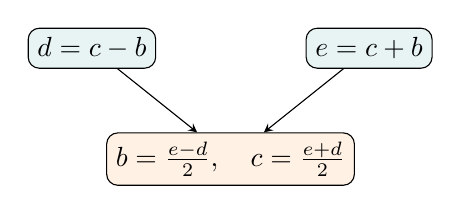
\begin{tikzpicture}[>=stealth,scale=.88]
\node[draw,fill=teal!9,rounded corners] (a) at (0,0){$d=c-b$};
\node[draw,fill=teal!9,rounded corners] (b) at (4,0){$e=c+b$};
\node[draw,fill=orange!10,rounded corners] (c) at (2,-1.6){$b=\frac{e-d}{2},\quad c=\frac{e+d}{2}$};
\draw[->] (a)--(c);\draw[->] (b)--(c);
\end{tikzpicture}

\end{center}
\medskip
任何正整数 $b,c$ 都对应唯一因数对 $(c-b,c+b)$。反过来，只要 $de=a^2$ 且因数对同奇同偶、$0<d<e$，代入 $b=(e-d)/2,c=(e+d)/2$ 就得到正整数解。两方向都成立，才说明没有遗漏。
\end{explanationbox}
\clearpage
\begin{explanationbox}
\textbf{\textcolor{CExplanation}{为什么一定要同奇同偶}}
\par\medskip
\begin{center}
% F090｜parity 原创简明教学示意图
\begin{tikzpicture}[>=stealth,scale=.92]
\node[draw,rounded corners,fill=orange!8] at (0,0){$d,e$ 一奇一偶};
\node at (3.3,0){$\Rightarrow$};
\node[draw,rounded corners,fill=teal!9] at (7,0){$\frac{e-d}{2}$ 不是整数};
\node at (3.7,-1.2){\small 因数配对必须检查同奇同偶};
\end{tikzpicture}

\end{center}
\medskip
因为 $e-d=2b$、$e+d=2c$ 都是偶数，$d,e$ 必须同奇同偶。若一奇一偶，算出的 $b$ 或 $c$ 会是半整数，不符合题意。
\end{explanationbox}
\clearpage
\begin{explanationbox}
\textbf{\textcolor{CExplanation}{固定直角边9的完整演示}}
\par\medskip
\begin{center}
% F090｜pairs 原创简明教学示意图
\begin{tikzpicture}[>=stealth,scale=.94]
\node[draw,rounded corners,fill=teal!8] (a) at (0,0){$9^2=81$};
\node[draw,rounded corners,fill=orange!8,align=center] (b) at (4.2,0){$1\times81$\\$3\times27$\\$9\times9$};
\node[draw,rounded corners,fill=teal!13,align=center] (c) at (8.5,0){$(9,40,41)$\\$(9,12,15)$\\$b=0$ 排除};
\draw[->,thick] (a)--(b);\draw[->,thick] (b)--(c);
\end{tikzpicture}

\end{center}
\medskip
$9^2=81$，按 $d<e$ 列出 $(1,81),(3,27),(9,9)$。前两组给 $(b,c)=(40,41)$、$(12,15)$；最后一组 $b=0$ 排除。因此恰有两组。
\end{explanationbox}
